\apendice{Documentación técnica de programación}

\section{Introducción}
Este documento técnico proporciona toda la información necesaria para que un desarrollador pueda instalar, ejecutar y mantener el programa.

Está dirigido a programadores, colaboradores o personal técnico que desee contribuir al proyecto, comprender su estructura interna o realizar mejoras y extensiones futuras. 
\section{Estructura de directorios}

En esta sección se describe la estructura jerárquica de carpetas empleada en el desarrollo del entorno, implementado en \textit{Unreal Engine}. La clasificación de los recursos se ha realizado de forma modular, separando claramente los elementos visuales, la lógica del juego, las interfaces de usuario y los activos reutilizables, con el objetivo de facilitar tanto el trabajo colaborativo como la futura evolución del sistema.

\begin{figure}[H]
    \centering
    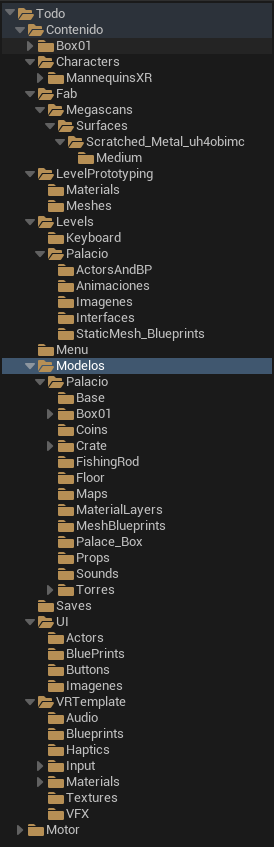
\includegraphics[scale=0.4]{../img/anexos/estructura_del_proyecto.png}
    \caption[ Estructura del proyecto]{Estructura del proyecto}
    \label{fig:estructura_del_proyecto}
\end{figure}

\subsection{Descripción de la estructura}

\texttt{Todo/} – Carpeta raíz del proyecto, contiene todos los activos y recursos del entorno de desarrollo en \textit{Unreal Engine}.

\begin{itemize}
  \item \texttt{Contenido/} – Carpeta principal de contenido dentro del editor de Unreal Engine.
  \begin{itemize}
    \item \texttt{Characters/} – Personajes utilizados en el entorno.
    \begin{itemize}
      \item \texttt{MannequinsXR/} – Modelos base y esqueletos optimizados para realidad virtual extendida.
    \end{itemize}
    \item \texttt{Fab/} – Carpeta que agrupa elementos descargados mediante el marketplace de Unreal.
    \begin{itemize}
      \item \texttt{Megascans/} – Repositorio de materiales escaneados de alta calidad.
      \begin{itemize}
        \item \texttt{Surfaces/} – Superficies específicas utilizadas en escenas.
      \end{itemize}
    \end{itemize}
    \item \texttt{LevelPrototyping/} – Elementos para diseño preliminar de niveles.
    \begin{itemize}
      \item \texttt{Materials/}, \texttt{Meshes/} – Materiales y mallas usados para prototipado.
    \end{itemize}
    \item \texttt{Levels/} – Niveles jugables o en desarrollo.
    \begin{itemize}
      \item \texttt{Keyboard/} – Nivel asociado al uso de teclado.
      \item \texttt{Palacio/} – Nivel principal del entorno virtual.
      \begin{itemize}
        \item \texttt{ActorsAndBP/} – Actores y \textit{Blueprints} usados en el nivel.
        \item \texttt{Animaciones/} – Animaciones de personajes u objetos.
        \item \texttt{Imagenes/} – Recursos gráficos.
        \item \texttt{Interfaces/} – Interfaces para interacción usuario-juego.
        \item \texttt{StaticMesh\_Blueprints/} – Mallas estáticas con lógica personalizada.
      \end{itemize}
    \end{itemize}
    \item \texttt{Menu/} – Elementos del menú principal de la aplicación.
    \item \texttt{Modelos/} – Modelos 3D usados en la aplicación.
    \begin{itemize}
      \item \texttt{Palacio/} – Carpeta con submodelos y utilidades específicas del entorno tipo palacio.
      \begin{itemize}
        \item \texttt{Base/}, \texttt{Box01/}, \texttt{Coins/}, \texttt{Crate/}, \texttt{FishingRod/}, \texttt{Floor/}, \texttt{Maps/}, \texttt{MaterialLayers/}, \texttt{MeshBlueprints/}, \texttt{Palace\_Box/}, \texttt{Props/}, \texttt{Sounds/}, \texttt{Torres/} – Subcarpetas con modelos, sonidos y elementos visuales del entorno.
      \end{itemize}
    \end{itemize}
    \item \texttt{Saves/} – \textit{Savegames} utilizados en el proyecto
    \item \texttt{UI/} – Interfaz de usuario.
    \begin{itemize}
      \item \texttt{Actors/}, \texttt{BluePrints/}, \texttt{Buttons/}, \texttt{Imagenes/} – Componentes visuales interactivos de la UI.
    \end{itemize}
    \item \texttt{VRTemplate/} – Plantilla base de \textit{Unreal} para proyectos VR.
    \begin{itemize}
      \item \texttt{Audio/}, \texttt{Blueprints/}, \texttt{Haptics/}, \texttt{Input/}, \texttt{Materials/}, \texttt{Textures/}, \texttt{VFX/} – Recursos multimedia, entradas hápticas, materiales, texturas y efectos visuales usados en VR.
    \end{itemize}
  \end{itemize}
  \item \texttt{Motor/} – Recursos internos del motor Unreal que no deben modificarse directamente.
\end{itemize}
\section{Manual del programador}
El presente manual está dirigido a los desarrolladores que trabajen en el mantenimiento, ampliación o comprensión del sistema.
\subsection{Instalaciones necesarias}

Para el desarrollo y despliegue del proyecto, se requieren las siguientes herramientas y plataformas:

\subsubsection*{\textit{Unreal Engine 5}}

\textit{Unreal Engine 5} es el motor principal utilizado para desarrollar el entorno de realidad virtual interactivo. Se ha elegido por su potencia gráfica, compatibilidad con \textit{VR} y soporte para programación en C++.

\begin{itemize}
    \item Página oficial de descarga: \href{https://www.unrealengine.com/download}{Unreal Engine}
    \item Versión utilizada en el proyecto: 5.4
\end{itemize}

\textbf{Pasos de instalación:}
\begin{enumerate}
    \item Crear una cuenta en \href{https://www.epicgames.com/site/es-ES/home}{\textit{Epic Games}}.
    \item Descargar el \textit{Epic Games Launcher}.
    \item Instalar \textit{Unreal Engine 5.4} desde el lanzador.
\end{enumerate}

\subsubsection*{\textit{Blender}}

\textit{Blender} se ha utilizado para el modelado y exportación de objetos 3D empleados en el puzle.

\begin{itemize}
    \item Página oficial de descarga: \href{https://www.blender.org/download/}{Blender}
    \item Versión utilizada en el proyecto: 3.6 LTS
\end{itemize}

\textbf{Pasos de instalación:}
\begin{enumerate}
    \item Descargar el instalador desde la página oficial.
    \item Ejecutar el archivo y seguir el asistente de instalación.
    \item Verificar la exportación en formato \texttt{.fbx} para su compatibilidad con Unreal Engine.
\end{enumerate}

\subsubsection*{\textit{Visual Studio 2022 Community}}

\textit{Visual Studio} es el entorno de desarrollo empleado para compilar y depurar el código C++ del proyecto.

\begin{itemize}
    \item Página oficial de descarga: \href{https://visualstudio.microsoft.com/es/}{Visual Studio}
    \item Edición recomendada: \textit{Community Edition}
\end{itemize}

\textbf{Componentes requeridos:}
\begin{itemize}
    \item \textit{Desarrollo para escritorio con C++}
    \item \textit{Herramientas de desarrollo para Unreal Engine}
\end{itemize}

\subsubsection*{\textit{Meta Quest Link}}

Para ejecutar el entorno en un dispositivo \textit{Meta Quest 2}, es necesaria la aplicación \textit{Meta Quest Link}, que permite conectar el visor al PC y ejecutar las escenas directamente desde Unreal Engine.

\begin{itemize}
    \item Página oficial de descarga: \href{https://www.meta.com/es-es/help/quest/1517439565442928/?srsltid=AfmBOoo5g0JE6USz6f9AFDuI3ggzFrRQl7LbQTSv9CvtSk7leU17CGWp}{Meta Quest Link}
\end{itemize}

\subsubsection*{\textit{GitLab}}

El código fuente del proyecto se encuentra alojado en un repositorio privado de \textit{GitLab}.

\textbf{Pasos para clonar el repositorio:}
\begin{enumerate}
    \item Abre una terminal y navega al directorio deseado.
    \item Ejecuta:
    
    \begin{small}
    \texttt{git clone https://gitlab.com/HP-SCDS/Observatorio/2024-2025/vrrecoverygym/
    ubu-vrrecoverygym}
    \end{small}
    \item Abre el proyecto desde el \textit{Epic Games Launcher} o desde Unreal Engine directamente.
\end{enumerate}

\subsection{Hardware utilizado}

El hardware mínimo necesario para desarrollar y ejecutar el proyecto incluye:

\begin{itemize}
    \item \textbf{PC de desarrollo} con las siguientes características recomendadas:
    \begin{itemize}
        \item Procesador: Intel i7 / AMD Ryzen 7 o superior.
        \item Memoria RAM: mínimo 16 GB.
        \item Tarjeta gráfica: NVIDIA RTX 3060 o superior.
        \item Almacenamiento: SSD de al menos 500 GB.
    \end{itemize}

    Estas especificaciones no son las mínimas, pero son las recomendadas para un desarrollo cómodo sobre el proyecto.
    
    \item \textbf{Dispositivo de realidad virtual:} \textit{Meta Quest 2} con conexión mediante \textit{Meta Quest Link}.
    \begin{itemize}
        \item Página oficial del producto: \href{https://www.meta.com/quest/meta-quest-2/}{Meta Quest 2}
        \item Requiere cable USB 3.0 compatible (recomendable por rendimiento) o conexión \textit{Wi-Fi} para \textit{Air Link}.
    \end{itemize}

    Existe la posibilidad de probar el proyecto con gafas de versiones superiores como las Meta Quest 3
    o 3s.
\end{itemize}

\section{Compilación y ejecución del proyecto}
Una vez el repositorio esté clonado, abre Unreal Engine y ve a \textit{Archivo > Abrir} proyecto, navega hasta la carpeta donde está el proyecto y abre el archivo .uproject.

\textbf{Verificación de dependencias}: Se recomienda verificar desde el menú \textit{Editar > Complementos} que los complementos \textit{OpenXR} y \textit{VictoryBPLibrary} estén activados. 

\subsection{Ejecución del proyecto}

Para ejecutar el proyecto directamente en el visor VR, es necesario:
    \begin{itemize}
        \item Tener correctamente configurado el entorno de desarrollo con el dispositivo.
        \item Conectar las gafas al PC mediante \textit{Air Link} o cable USB-C a traves de la aplicación Meta Quest Link.
        \item Presionar el botón \textit{Play} y seleccionar la opción \textit{VR Preview}.
    \end{itemize}

El nivel por el que empezarás es el que esté abierto, por defecto es \textit{Level\_Start} que es el primer nivel del juego, si necesitas hacer pruebas sobre otro nivel tan solo ábrelo en el editor y sigue los mismos pasos. 


\section{Pruebas del sistema}

Las pruebas del sistema constituyen una fase esencial para validar el correcto funcionamiento del proyecto, detectar errores y verificar que se cumplen los objetivos definidos. En el caso de un entorno de rehabilitación motriz en realidad virtual, estas pruebas incluyen tanto comprobaciones técnicas como pruebas de experiencia de usuario.

A continuación, se describen los principales tipos de pruebas realizadas:

\subsection{Pruebas funcionales}

Estas pruebas tienen como objetivo verificar que las distintas funcionalidades del sistema operan correctamente, de acuerdo con los requisitos establecidos.

\begin{itemize}
    \item \textbf{Carga del entorno}: Se prueba que el entorno se carga sin errores y todos los elementos visuales aparecen correctamente.
    
    \item \textbf{Interacción con objetos}: Se verifica que el usuario puede manipular los objetos mediante controladores \textit{VR} (agarre, colocación, rotación, etc.).
    
    \item \textbf{Seguimiento de manos y controladores}: Se comprueba que el sistema reconoce correctamente los movimientos del usuario, así como la respuesta háptica.
    
    \item \textbf{Detección de finalización de tareas}: Se prueban los mecanismos de validación de los puzles o ejercicios, asegurando que el sistema reconoce cuándo se ha completado correctamente una tarea.
    
\end{itemize}

\subsection{Pruebas de rendimiento}

Se evalúa el comportamiento del sistema bajo condiciones normales de uso, garantizando una experiencia fluida y sin interrupciones:

\begin{itemize}
    \item \textbf{Tasa de fotogramas por segundo (FPS)}: Se mide el rendimiento con herramientas con la herramienta \textit{Unreal Insights}. buscando mantener al menos 72 FPS en el visor VR.
    \item \textbf{Consumo de memoria}: Se evalúa el uso de recursos para asegurar que el sistema no sobrepasa los límites del \textit{hardware}.
    
    \item \textbf{Tiempos de carga}: Se comprueba que el inicio del entorno y las transiciones entre niveles (si los hubiera) no introducen retardos perceptibles.
\end{itemize}

\begin{figure}[h]
	\caption[Ejemplo de telemetria]{Ejemplo de telemetria del proyecto con \textit{Unreal Insights}}
	\centering
	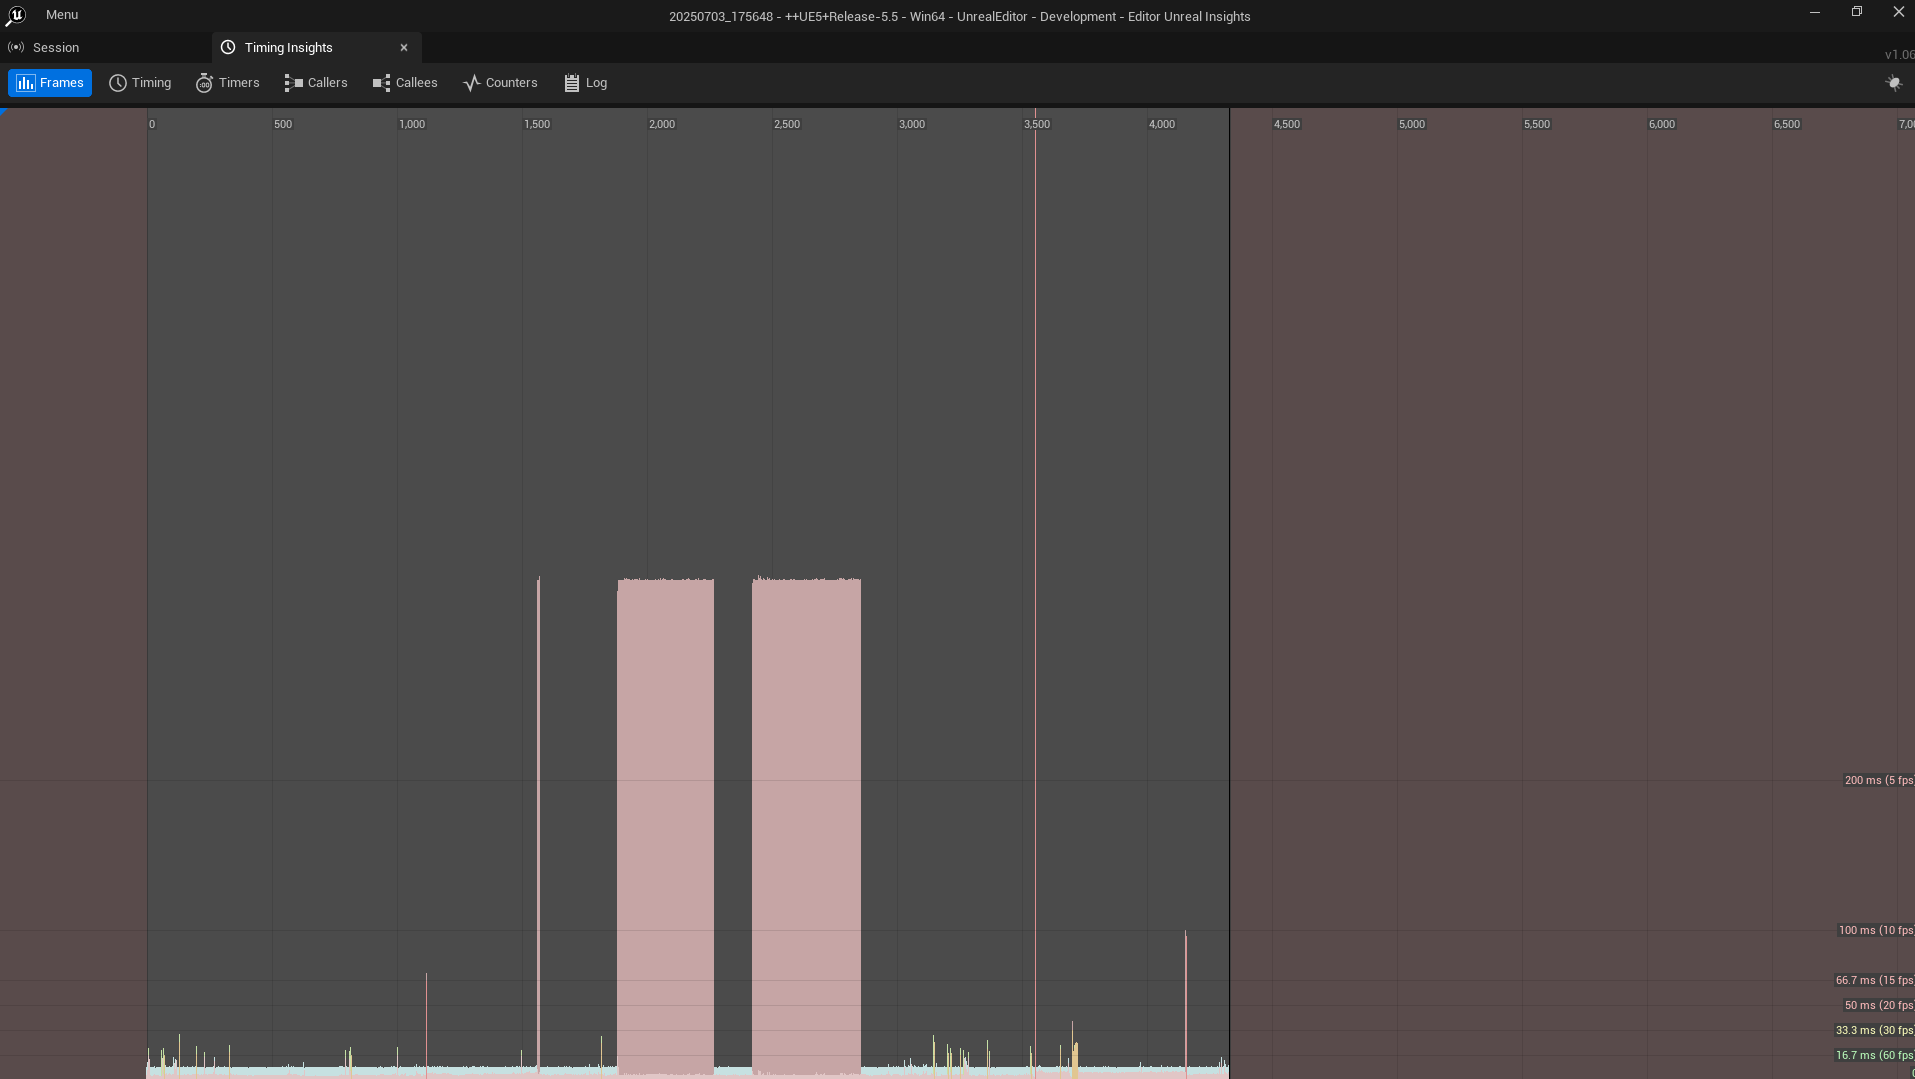
\includegraphics[width=\textwidth]{../img/anexos/ejemplo_telemetria_unreal.png}
	\label{b:telemetria_unreal}
\end{figure}

\subsection{Pruebas de usuario}

Se planifican sesiones de prueba con usuarios colaboradores, objetivo de evaluar:

\begin{itemize}
    \item \textbf{Accesibilidad}: Evaluar si el sistema puede ser utilizado de forma sencilla por personas con movilidad reducida en extremidades superiores.
    
    \item \textbf{Usabilidad}: Identificar barreras de uso, errores de diseño o elementos confusos.
    
    \item \textbf{Recogida de feedback}: A través de entrevistas, se recoge información cualitativa sobre la experiencia del usuario y posibles mejoras.
    
\end{itemize}

\subsection{Registro de incidencias}

Durante todas las fases de prueba, se utiliza un sistema de control de incidencias mediante \textit{GitLab Issues} y documentando su resolución dentro del flujo de trabajo de \textit{SCRUM}.

\subsection{Automatización de pruebas}

En esta fase del desarrollo se han priorizado pruebas manuales debido al carácter interactivo y centrado en la experiencia de usuario del sistema.

\begin{table}[H]
    \centering
    \begin{tabular}{|p{4cm}|p{5cm}|p{5cm}|}
        \hline
        \textbf{Caso de prueba} & \textbf{Acción realizada} & \textbf{Resultado esperado} \\
        \hline
        Registro de nuevo usuario & Introducir datos válidos (nombre) en la interfaz de inicio. & El sistema registra al usuario y redirige a la pantalla de menú principal. \\
        \hline
        Registro de usuario incorrecto& Introducir un nombre con menos de 3 caracteres o más de 20. & El sistema muestra un mensaje de error y no permite el registro. \\
        \hline
        Crear nuevo puzle & Se crea un nuevo puzle desde la interfaz  & Se carga el entorno principal y se crea un nuevo \textit{savegame} con los datos de la creación. \\
        \hline
        Interacción con un puzle & Se realiza y completa un puzle. & Todas los pasos funcionan correctamente y  los datos son guardados correctamente.\\
        \hline
        Integridad de los datos & Borrar y crear puzles. & Los datos de los puzles son persistentes y se asignan bien los indices. \\
        \hline
        Funcionalidad mano derecha e izquierda & Realizar acciones con la interfaz y el puzle con ambas manos & Ambas manos deben poder realizar todas las acciones disponibles en el programa. \\
        \hline
    \end{tabular}
    \caption{Casos de prueba manuales en el proyecto}
    \label{tabla:casos-prueba-vr}
\end{table}